%%%%%%%%%%%%%%%%%%%%%%%%%%%%%%%%%%%%%%%%%%%%%%%%%%%%%%%%%%%%%%%%%%%%%%%%
%%%%%%%%%%%%%%%%%%%%%%%%%%%%% EVALUATION %%%%%%%%%%%%%%%%%%%%%%%%%%%%%%%
%%%%%%%%%%%%%%%%%%%%%%%%%%%%%%%%%%%%%%%%%%%%%%%%%%%%%%%%%%%%%%%%%%%%%%%%
In this chapter, we present the results of the experimental evaluation of our work. We assess the usability of the BNCE TGG formalism, by comparing the size of the BNCE grammars for five example transformations with their equivalent grammars written in standard TGG, and the performance of our implemented transformer, by measuring the average runtime took to transform some model instances for our example transformations.

%%%==================================================================%%%
%%%%%%%%%%%%%%%%%%%%%%%%%%%%%% USABILITY %%%%%%%%%%%%%%%%%%%%%%%%%%%%%%%
%%%==================================================================%%%
\section{Usability}
In order to evaluate the usability of the proposed BNCE TGG formalism, we compare the amount of rules and elements (vertices, edges and mappings) we needed to describe some typical model transformations in BNCE TGG and in standard TGG without application conditions. Table \ref{tab:formalism-eval} presents these results. Each line displays the results for one different transformation, the first and second columns provide the amount of rules and elements of the standard TGG specifications and the third and forth columns the amount of rules and elements of the BNCE TGG specifications, respectively. The size of the smaller specification for each transformation is printed in bold. If a transformation could not be specified with a formalism, the respective cells are marked with a dash (-). The three last lines indicate the sum, the arithmetic average and the median of the amount of rules and elements of each formalism for the compared transformations, respectively.

In general, we judge that the smaller a grammar is, the better its usability is. In this sense, our approach outperforms the baseline in one transformation case and can specify another case, that we could not specify with standard TGG at all. In addition, judging by the measures of total and average, BNCE TGG perform significantly better than the considered baseline. This observation is though not conclusive, because the negative result of the standard TGG is strongly influenced by one studied case in which it performs specially worse, this is made clear by the median of the grammar sizes. Insofar, we cannot claim that our evaluation has a strong statistical validity, for the studied transformations are not very representative in general and we cannot guarantee that these are the smallest grammars that describe the desired transformations. Nonetheless, this results should demonstrate the potential of our approach.

%TODO: Make clear that two last transformations were written with PAC BNCE TGG
\begin{table}[h]
	\centering
	\caption{Results of the usability evaluation of the BNCE TGG formalism in comparison with the standard TGG for the model transformation problem}
	\label{tab:formalism-eval}
	\begin{tabular}{l r r r r }
		\hline
										& \multicolumn{2}{c}{Standard TGG}	& \multicolumn{2}{c}{BNCE TGG}\\
		Transformation 					& Rules 		& Elements 		& Rules 		& Elements\\
		\hline
		\emph{Pseudocode2Controlflow}	& 47			& 1085			& \textbf{7}	& \textbf{185}	\\
		\emph{BTree2XBTree}				& \textbf{4}	& \textbf{50}	& 5				& 80 			\\
		\emph{Star2Wheel}				& -				& -				& \textbf{6} 	& \textbf{89} 	\\
		\emph{Class2Database}			& \textbf{5}	& \textbf{80}	& 9 			& 117  			\\
		\emph{Statemachine2Petrinet}	& \textbf{5}	& \textbf{114}	& 7				& 131 			\\
		\hline
		Total							& 61 			& 1329			& \textbf{28}	& \textbf{513}	\\
		Average							& 15.25 		& 332.25		& \textbf{7}	& \textbf{128.25}\\
		Median							& \textbf{5}	& \textbf{97}	& 7				& 124			\\
		\hline
	\end{tabular}
\end{table}

In the case of \emph{Pseudocode2Controlflow}, our proposed approach shows a clear advantage against the standard TGG formalism. We judge that, similarly to what happens to programming languages, this advantage stems from the very nested structure of \emph{Pseudocode} and \emph{Controlflow} graphs. That is, for instance, in rule the $r_2$ of this TGG (see Example \ref{ex:pseudocode2controlflow}), a node in a positive branch of an $if$-labeled vertex is never connected with a node in the negative branch. This disjunctive aspect allows every branch to be defined in the rule (as well as effectively parsed) independently of the other branch. This characteristic makes it possible for BNCE TGG rules to be defined in a very straightforward manner and reduces the total amount of elements necessary.

In addition to that, the use of non-terminal symbols gives BNCE TGG the power to represent abstract concepts very easily. For example, whereas the rule $r_1$ encodes, using only few elements, that after each \emph{action} comes any statement $A$, which can be another \emph{action}, an \emph{if}, a \emph{while} or nothing (an empty graph), in the standard TGG without application condition or any special inheritance treatment, we need to write a different rule for each of these cases. For the whole grammar, we need to consider all combinations of \emph{actions}, \emph{ifs} and \emph{whiles} in all rules, what causes the great amount of rules and elements.

The \emph{BTree2XBTree} transformation consists of lifting binary trees to graphs by adding edges between siblings. In this scenario, our approach performed slightly worse than TGG. The \emph{Star2Wheel} transformation consists of transforming star graphs, which are complete bipartite graphs $K_{1,k}$, with the partitions named center and border, to wheel graphs, that can be constructed from star graphs by adding edges between border vertices to form a minimal cycle. We could not write this transformation in standard TGG, specially because of the rules' monotonicity (see Definition \ref{def:stgg}). That is, we missed the possibility to erase edges in a rule, feature that we do have in the semantics of BNCE TGG through the embedding mechanism.

%TODO: Comment the last 2 TGGs, not yet commented

In summary, our experimental usability evaluation does not allow the drawing of definitive conclusions concerning the usability of the compared formalisms, although it provides strong positive evidences about the BNCE TGG's potential. In addition, we cannot affirm which of the two formalisms is more expressive, for that would require a deeper theoretical analysis that include the characterization of an order of grammars. That is, in order to say that a family of grammars is more expressive than other, we would need to find a containment relation between the former and the latter, what does not seem to be trivial.

Positively, we highlight the capacity of BNCE TGG to specify very compactly transformations between graphs for whose label sets there exists some kind of inheritance relation. In other words, models in which element types' undergo a hierarchical structure fit BNCE TGG well. That is particularly common for behavioral models of software systems, therefore, we claim that our approach suits well, for example, the automatic generation of source-code out of graphic models.

%TODO: Add citation for TGG with AC
Regarding the \emph{Star2Wheel} transformation, we believe that it could be written with standard TGG augmented with application conditions (AC). In which case, BNCE TGG can be seen as an alternative to TGG with AC, what makes it, in circumstances where AC are not wished, specially applicable.

Negatively, the lack of context imposed by the pure BNCE TGG demand the use of PAC for some transformations. Although we prove in Theorem \ref{thm:one_d_enough_pac} that the PAC mechanism can be used safely for the solving of the model transformation problem, we suppose that its application can be perceived as cumbersome in some situations, especially with the occurrence of multiple PAC, that we did not include in our evaluation.

%%%==================================================================%%%
%%%%%%%%%%%%%%%%%%%%%%%%%%%%% PERFORMANCE %%%%%%%%%%%%%%%%%%%%%%%%%%%%%%
%%%==================================================================%%%
\section{Performance}
%TODO: Cite eMoflon
%TODO: Change X and Y by real references
For the purpose of evaluating the performance of our implemented transformation algorithm, we measure the runtime taken by it to transform various input graph of various sizes for the same five example transformations from the previous section. We provide the average runtime of our implementation in comparison with the standard TGG transformer \emph{eMoflon}. Thereby, we discriminate inputs that generate a deeper or a shallower parsing tree and depict these results in Figures X to Y, the x-axis represents the size of the inputs, the y-axis the runtime in seconds and the various lines the arithmetic average runtime for the two classes of inputs (Deep and Shallow) on the two transformer implementations (BNCE and eMoflon).

%TODO: Talk more about configuration. Talk about eMoflon...

\begin{figure}
	\centering
	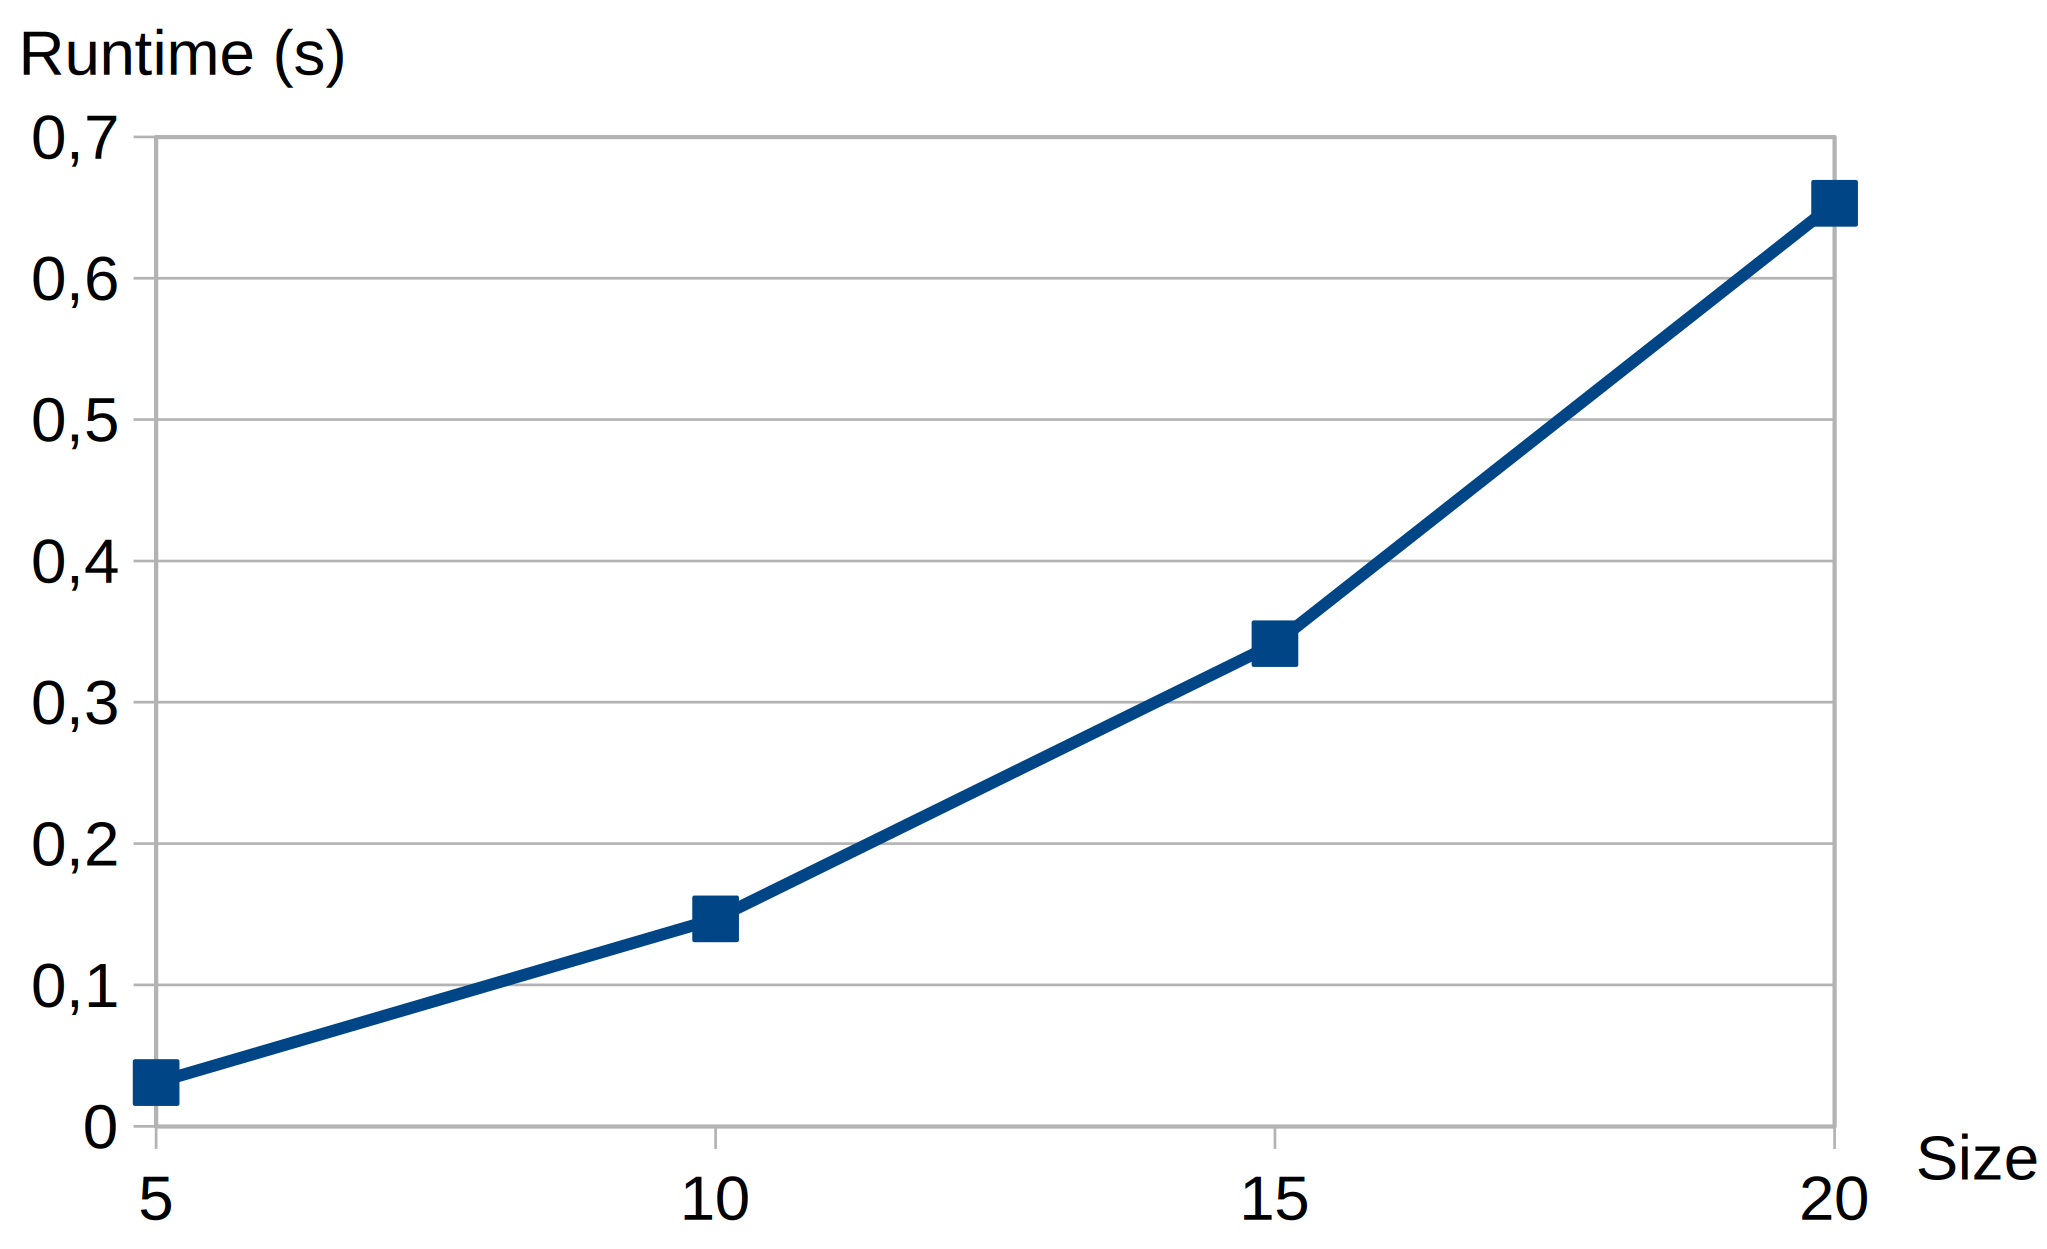
\includegraphics[width=.5\textwidth]{figures/performance/star2wheel}
	\caption{...}
	\label{fig:performance-star2wheel}
\end{figure}

\begin{figure}
	\centering
	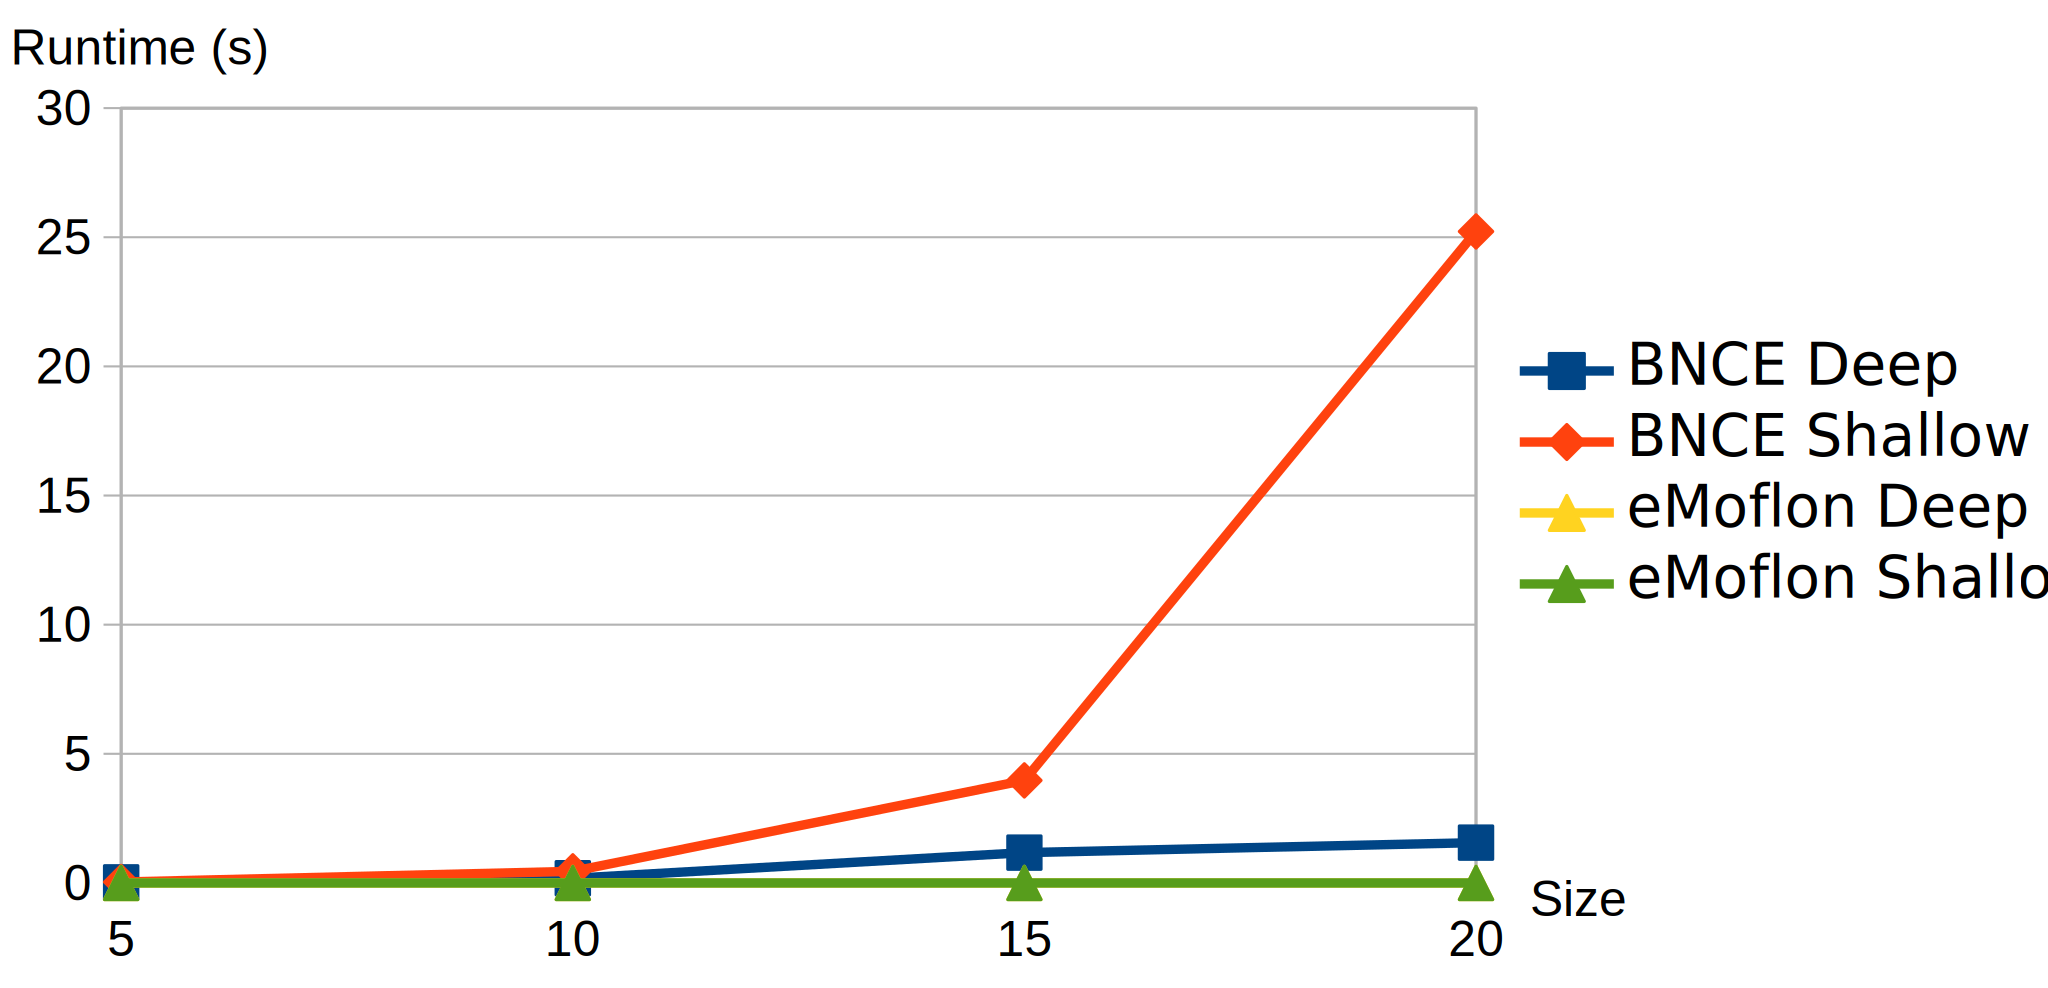
\includegraphics{figures/performance/pseudocode2controlflow}
	\caption{...}
	\label{fig:performance-pseudocode2controlflow}
\end{figure}

%TODO: Positive and negative aspects of the proposed approach. Cases where it specially works good and bad. Best case. Worst case in regard to parsing tree structure. Average case

Furthermore, we also report on the runtime for forward and backward batch transformations in a Intel Core i3 2.3GHz 4x 64bit with 4GB RAM. The standard TGG version of the transformations were executed using the eMoflon Tool %\cite{leblebici2014developing}.
%TODO: Which implementation details: threads, strategy, etc

Regarding the worst-case time complexity of our model transformer, it is clear that it is linear on the size of the source model for the step \emph{Ecore to Graph} and it is polynomial in the size of the TGG model for the step \emph{NP Normalization}. For the step \emph{Production}, the time complexity is linear on the length of the derivation, which in turn is linear on the size of the source graph. And, ultimately, \cite[p. 160]{rozenberg1986boundary} demonstrates that the parser finishes in polynomial time for degree-bounded connected source graphs. Thus, the worst-case time complexity of the model transformer is also polynomial for this case.

%TODO: Maybe need to explain better these factors, special the fact that bup the internal complexity is fast because the subsets are bounded by maxr(G)
In particular, the parser's complexity dominates the total complexity and can be roughly described by the multiplication of two factors: the number of loop iterations executed until the desired final zone vertex is found (Lines 4 to 14 in Algorithm \ref{alg:parsepac}) and the number of operations necessary to find the derivations for a handle (Lines 5 to 13 in Algorithm \ref{alg:parsepac}). The latter is clearly a function on the size of the grammar, that is the number of rules and the right-hand sides' sizes, that are considered to be fixed, for handles bounded by the greatest right-hand side. The former is the size of the $bup$ set, which in turn is polynomial in the size of the source graph, for a degree-bounded connected graph \cite[p. 161]{rozenberg1986boundary}.

%TODO: Space complexity. NLOG? Look in paper about efficiency and complexity of Kim.. Say also that much memory is used by us in the practice; search space with parsing trees and bup sets. space complexity for production is linear on source graph size


%TODO: Which is the averga, best and worst case
%TODO: Write about top-down alternative
%TODO: Say that embeddings are complicated
%TODO: "Generating Efficient Parsers for HR grammars", Cite s_78 for evaluation of HRGs
%TODO: HR are too few expressive